\documentclass{article}

\usepackage{listings}
\usepackage{xcolor}
\usepackage{xeCJK}
\usepackage{pdfpages}
\lstdefinelanguage{b2b}
{
    morekeywords={Title, Author, Ack, Label, Name, Path, textcolor, and},
    sensitive=false,
    morecomment=[l]{//},
    morecomment=[l]{*},
    morecomment=[s]{/*}{*/},
    morestring=[b]",
}
\lstdefinelanguage{LaTeX}[LaTeX]{TeX}{
  morekeywords={begin,end,title,author,date,maketitle,section,textbf,switchcolumn,sidebyside,endbyend,textwidth,linewidth,toprule,midrule,bottomrule,includegraphics,subsection,lstinputlisting,subfigure,CrossColumnText,aicescovertitle,aicescoverauthor,aicescoverack,aicescoverpage,textcolor,includepdfset,includepdf},
}
\newfontfamily\courier{Courier New}
\lstset{linewidth=\linewidth,
    numbers=left, %设置行号位置 
    basicstyle=\small\courier,
    numberstyle=\tiny\courier, %设置行号大小  
    keywordstyle=\color{blue}\courier, %设置关键字颜色  
    %identifierstyle=\bf,
    commentstyle=\it\color{gray}\courier, %设置注释颜色 
    stringstyle=\it\color[RGB]{128,0,0}\courier,
    %framexleftmargin=10mm,
    frame=single, %设置边框格式  
    backgroundcolor=\color[RGB]{245,245,244},
    %escapeinside=``, %逃逸字符(1左面的键),用于显示中文  
    breaklines, %自动折行
    columns=fullflexible,
    extendedchars=false, %解决代码跨页时,章节标题,页眉等汉字不显示的问题  
    %xleftmargin=2em,xrightmargin=2em, aboveskip=1em, %设置边距  
    tabsize=4, %设置tab空格数  
    showspaces=false %不显示空格  
} 

\usepackage{graphicx}
\usepackage{float}
\usepackage{shortvrb}
\MakeShortVerb|

\usepackage[colorlinks]{hyperref}
\title{Bib2Book -- A program to put your bibliographies together\footnote{Project link: \url{https://github.com/Hailin-Jing/Bib2Book}}}
\author{WANG Hailin\thanks{Tongji University, School of Civil Engineering, Department of Geotechnical Engineering, Github: \url{https://github.com/Hailin-Jing}, Homepage: \url{https://hailin.blog}}}
\date{\today}

\begin{document}
    \maketitle

    \section{Installation}

    |Bib2Book| is a program to put your bibliographies together. 

    \subsection{Requirements}

    Before installtion, some necessary environments are needed.

    \paragraph{Cormorant Garamond Font}

    The program uses the |Cormorant Garamond| font. Unzip the release file, install fonts inside the |fonts/cormorant-garamond| directory.

    \paragraph{The \LaTeX Environment}

    The program uses \href{https://www.latex-project.org}{\LaTeX} to generate files, so you need to install one of the \LaTeX distributions: \href{http://www.tug.org/texlive}{TeX Live} (recommended), \href{http://www.ctex.org/HomePage}{C\TeX}. Check if the environment variables are configured correctly.

    \subsection{Installation}

    Unzip the release file, click |Bib2Book_Setup.exe| to install, follow the instructions to finish the installation.

    \clearpage

    \section{Usage}

    The program's interface is shown in Figure \ref{fig:interface}.
    \subsection{Interface}
    \begin{figure}[htb]
        \centering
        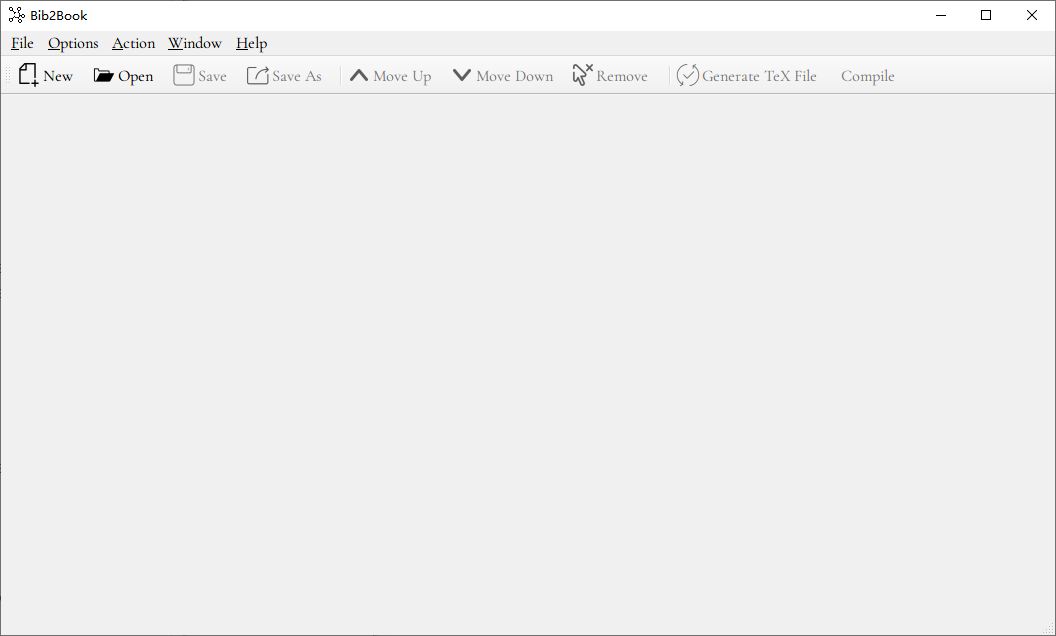
\includegraphics[width=\textwidth]{figures/interface.png}
        \caption{The program's interface}
        \label{fig:interface}
    \end{figure}

    \subsection{Create a Project}

    Click |New| button in the toolbar or in the |File| menu, and click |Save| button to save the project file, the name of the project file is ended by |.b2b|. Once the project file is saved successfully, next time you can just double-click the file or drag the file to the |Bib2Book| window or click the |Open| button to open it.

    \subsection{Provide your book information}
    Input the title, Authors, and footnote which will appear on the cover page, and provide documents that you want to add to the book. Double-click the |PDF| file to add it to your document-list, and you can define a label for each document and it will appear on the contents page to emphasize what this document is mainly about, the default value is a sorted number. Also, you can drag your |PDF| files in your explorer to the document-list section. You can click the |Move Up|, |Move Down|, and |Remove| button to manage your document-list.

    \begin{figure}[htb]
        \centering
        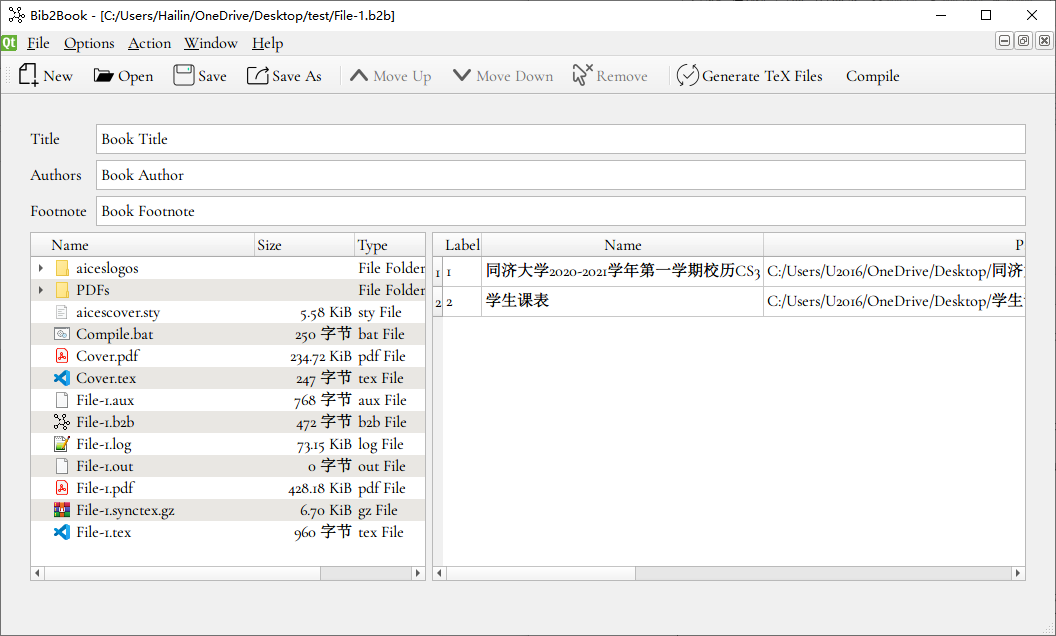
\includegraphics[width=\textwidth]{figures/project.png}
        \caption{Provide your book information}
        \label{fig:information}
    \end{figure}

    \section{Generate your book file}

    Once you finish managing your document-list of your book, you can click the |Generate TeX file| button to generate \TeX files of your book. Then click |Compile| button to compile it to |PDF| file, you must install one of the \LaTeX\ distributions to finish this step. When finished, the directory of the |PDF| will be opened automatically.

    \section{The Project file}

    This the format of the |Bib2Book| project file. You can simply write the |.b2b| file according to this format and change the suffix to |.b2b|.

\begin{lstlisting}[language=b2b, columns=fixed]
******************* Titlepage Information *******************
Title      = Book Title
Author     = Book Author
Ack        = Book Footnote

***************** Biblipgraphies Information *****************
// The symbol ``#'' indicates that this line is a record line.
     && Label   && Name   && Path // Header
  #  && Label-1 && Name-1 && Path-1 
  #  && Label-2 && Name-2 && Path-2
  #  ...
\end{lstlisting}

\section{\TeX\ files}

This is the \TeX\ files the program generated.\medskip

\noindent\textbf{Cover \TeX\ File:}

\begin{lstlisting}[language=LaTeX, columns=fixed]
% Cover TeX file
\documentclass{article}

\usepackage{aicescover}
\usepackage{xeCJK}
\usepackage{hyperref}

\begin{document}

	\aicescovertitle{Book Title}
	\aicescoverauthor{Book Author}
	\aicescoverack{Book Footnote}

	\aicescoverpage
\end{document}

\end{lstlisting}
\medskip
\noindent\textbf{Main \TeX\ File:}
\begin{lstlisting}[language=LaTeX, columns=fixed]
% Main TeX file
\documentclass[12pt]{book}

\usepackage{pdfpages}
\usepackage{hyperref}
\usepackage{xeCJK}
\usepackage{xcolor}
\usepackage[top=2cm, bottom=2cm, left=4cm, right=3cm]{geometry}
\pagestyle{empty}

\tolerance=1
\emergencystretch=\maxdimen
\hyphenpenalty=10000
\hbadness=10000

\begin{document}

	
\includepdf{Cover.pdf}
	\cleardoublepage

	\begin{center}
		\bfseries\centering\Large Table of Contents
	\end{center}
	\par

	\begin{itemize}
		\item[\textcolor{red}{Label-1}] Name-1 \hfill\textcolor{red}{\pageref{bib:1}}
		\item[\textcolor{red}{Label-2}] Name-2 \hfill\textcolor{red}{\pageref{bib:2}}
	\end{itemize}
	\cleardoublepage

	\includepdfset{pagecommand={\thispagestyle{headings}}}
	\setcounter{page}{1}

	\label{bib:1}
	\includepdf[pages=1-last]{PDFs/PDF-name-1.pdf}
	\label{bib:2}
	\includepdf[pages=1-last]{PDFs/PDF-name-2.pdf}

\end{document}
\end{lstlisting}

\section{Notes}

Some notes should be pointed out.
\begin{itemize}
    \item You can only choose |PDF| files.
    \item Some |PDF| files that downloaded from \href{https://cnki.net/}{cnki} may be encrypted, errors may occur when compiling or blank page may appear in the |PDF| file.
\end{itemize}

\section{Example}

This is a example of a |.b2b| file. You can find the project in \href{https://github.com/Hailin-Jing/Bib2Book/tree/main/release/documentation/example}{here}.

\lstinputlisting[language=b2b, columns=fixed]{example/example.b2b} 

\end{document}